
An alternate fit is performed which combines the WZ + 1-jet and WZ + 2-jet samples rather than fitting them independently. This is done primarily as a cross-check of the nominal analysis, to see if measuring 1-jet and 2-jet events separately and combining them gives drastically different results than measuring them together. 

For this study, three signal templates, WZ + $b$, WZ + $c$ and WZ + light, are fit to data, and the systematics accounting for migrations between 1-jet and 2-jet bins are removed. All other background and nuiscance parameters remain the same as the nominal fit. 

The measured $\mu$ value for WZ + $b$ is  $\mu = 1.00^{+0.30}_{-0.29}(stat)^{+0.25}_{-0.23}(sys)$, with a significance of 2.8$\sigma$, and the uncertainty on WZ + $c$ is $\mu = 1.00\pm 0.12 (stat)\pm 0.13 (sys)$. This is compared to combined uncertainty of $\mu = 1.00^{+0.32}_{-0.30}(stat)^{+0.24}_{-0.23}(sys)$ for WZ + $b$ when 1-jet and 2-jet events are measured separately and then combined.

A post-fit summary plot of the fit regions is shown in Figure \ref{fig:fit_results_inc}: 

\begin{figure}[H]
    \center
    \includegraphics[width=.9\linewidth]{sys_inclusive/Plots/Summary_postFit.png}
    \caption{Post-fit summary of the 1-jet fit regions.}
    \label{fig:fit_results_inc}
\end{figure}

The impact of the most significant sources of systematic uncertainties on the measurement of WZ + $b$ is summarized in Table \ref{tab:systematics_inc}. 

\begin{table}[H]
    \centering
    \begin{tabular}{l|cc}
        \hline\hline
        Uncertainty Source & \multicolumn{2}{c}{$\Delta \mu$ }  \\
        \hline
        WZ + light cross-section & 0.13 & -0.12 \\
        WZ + $c$ cross-section & -0.10 & 0.12 \\
        Jet Energy Scale & 0.08 & 0.13 \\
        tZ cross-section & -0.10 & 0.10 \\
        Jet Energy Resolution & -0.10 & 0.10 \\
        Luminosity & -0.08 & 0.09 \\
        Other Diboson + b cross-section & -0.07 & 0.07 \\
        Flavor tagging & 0.05 & 0.05 \\
        $t\bar{t}$ cross-section & -0.05 & 0.05 \\
        WZ cross-section - QCD scale & -0.04 & 0.03 \\
        \hline
        Total Systematic Uncertainty & 0.28 & 0.32 \\
        
        \hline\hline
    \end{tabular}
    \caption{Summary of the most significant sources of systematic uncertainty on the measurement of $WZ+b$ with one or two associated jets.}
    \label{tab:systematics_inc}
\end{table}

The ranking and impact of those nuisance parameters with the largest contribution to the overall uncertainty is shown in Figure \ref{fig:ranking_inc}.

\begin{figure}[H]
    \centering
    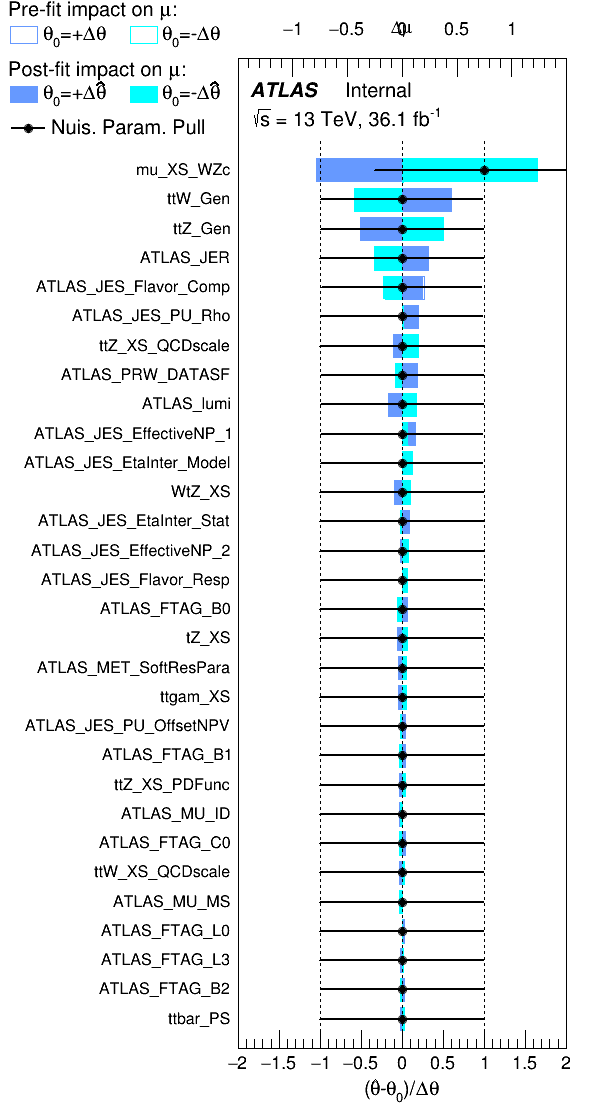
\includegraphics[width=0.7\linewidth]{sys_inclusive/Ranking.png}
    \caption{Impact of systematic uncertainties on the signal-strength of $WZ$ + b for events with one or two jets}
    \label{fig:ranking_inc}
\end{figure}

